\section{Resultados}
%Deben incluir los resultados de los experimentos, utilizando el formato más adecuado
%para su presentación. Deberón especificar claramente a qué experiencia corresponde
%cada resultado. No se incluirán aquí corridas de máquina. Algo fundamental en su
%aprendizaje en la materia es la presentación de resultados de forma clara y concisa para
%el lector.

\subsection{Eliminar sanguijuela}
\subsubsection{Experimento para Hipótesis 1}
Se modelaron 3 instancias, todas con los mismos valores de altura, ancho, granularidad, y cantidad de sanguijuelas. Lo único que se modifico en cada instancia fue el radio de estas últimas, principalmente con la idea de que:
 \begin{itemize}
    \item 1° Instancia = Todas sanguijuelas unitarias.
    \item 2° Instancia = Mitad sanguijuelas unitarias, mitad no unitarias.
    \item 3° Instancia  = Todas sanguijuelas no unitarias.
 \end{itemize}
 La temperatura de las sanguijuelas no es relevante al experimento, ya que no nos agrega nada saber la temperatura del punto crítico al mismo, y por simplicidad las mismas fueron ubicadas en posiciones múltiplos de la granularidad \\


Los resultados obtenidos fueron los siguientes:

\begin{figure}[H]
    \centering
    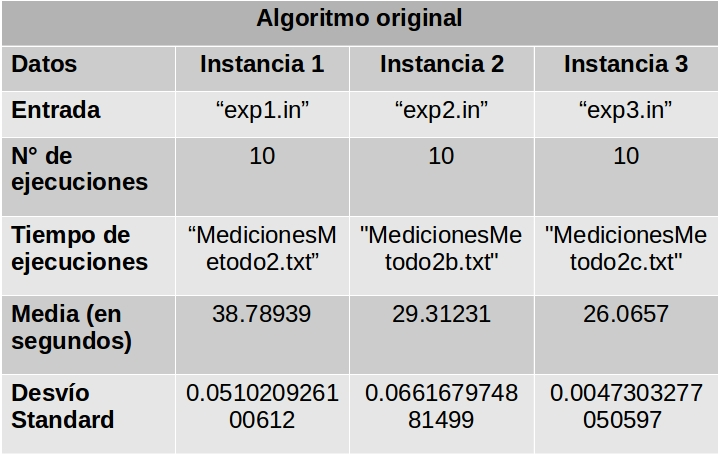
\includegraphics[scale=0.6]{graphs/tablaOriginal.jpg}
    \end{figure}
        
        
    \begin{figure}[H]
    \centering
    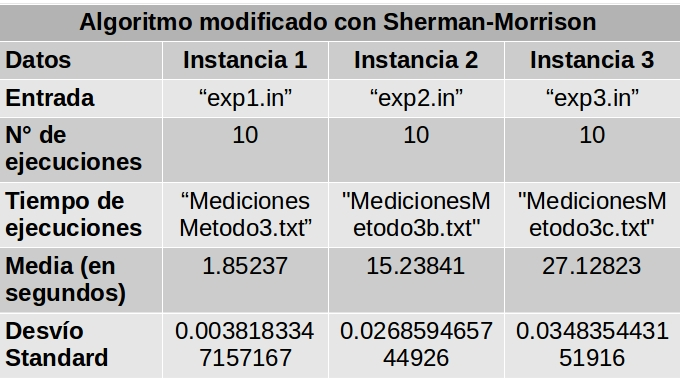
\includegraphics[scale=0.6]{graphs/tablaSherman.jpg}
    \end{figure}
        
        
 (Los archivos de entrada y los tiempos de corridas se puede encontrar en Experimentos/Experimento3).


    \begin{figure}[H]
    \centering
    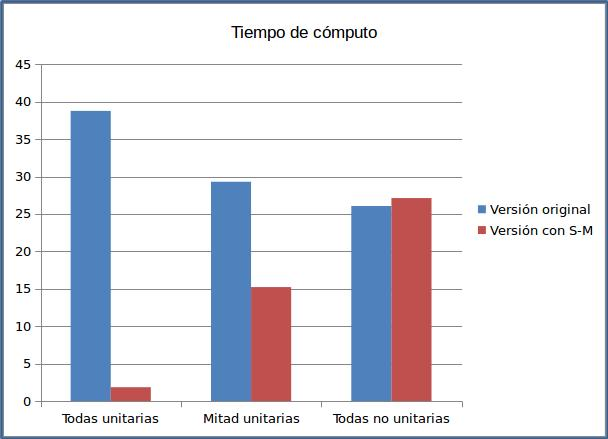
\includegraphics[scale=0.6]{graphs/graficoExp1.jpg}\caption{Gráfico obtenido de los valores de la media del tiempo de cada ejecución}
    \end{figure}
    
    
    
\subsubsection{Experimento para Hipótesis 2}
    Se modelaron 3 instancias, todas con los mismos valores de altura, ancho, cantidad de sanguijuelas, modificando la granularidad en cada una. El radio de las sanguijuelas se genero pseudoaleatoriamente con MATLAB en un rango posible de 0.1 a 16. Se eligió este rango para que el experimento sea más representativo con las granularidades elegidas para experimentar. Por simplicidad, las mismas fueron ubicadas en posiciones múltiplos de 16. Las instancias son las siguientes:
    
     \begin{itemize}
    \item 1° Instancia = Granularidad 8
    \item 2° Instancia = Granularidad 4
    \item 3° Instancia  = Granularidad 2
 \end{itemize}
 
  La temperatura de las sanguijuelas no es relevante al experimento, ya que no nos agrega nada saber la temperatura del punto crítico al mismo.
  
  Los resultados obtenido fueron los siguientes:
  
     \begin{figure}[H]
    \centering
    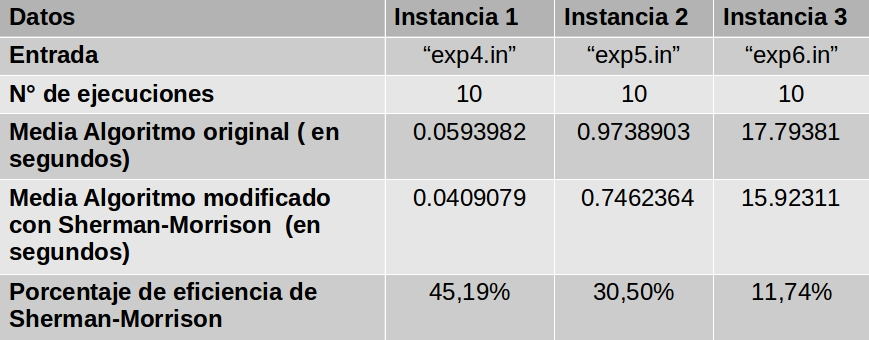
\includegraphics[scale=0.5]{graphs/grafico3.jpg}
    \end{figure}\
        
         (Los archivos de entrada y los tiempos de corridas se puede encontrar en Experimentos/Experimento3).


    \begin{figure}[H]
    \centering
    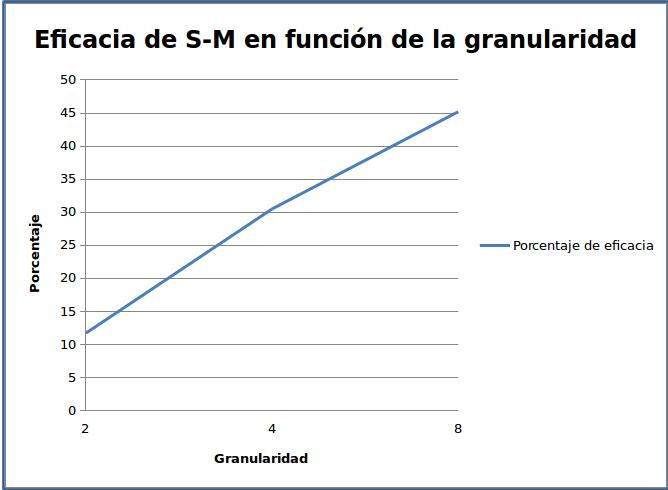
\includegraphics[scale=0.6]{graphs/graf.jpg}\caption{Gráfico obtenido de los valores del porcentaje de eficiencia del algoritmo con Sherman-Morrison comparándolo con el algoritmo original en función de la granularidad.}
    \end{figure}